\documentclass[11pt,twocolumn]{article}

\PassOptionsToPackage{hyphens}{url}
\usepackage{iftex}
\usepackage[margin=0.72in]{geometry}
\usepackage{graphicx}
\usepackage[hyphens]{url}
\usepackage{booktabs}
\usepackage{amsmath}
\usepackage{array}
\usepackage[hidelinks]{hyperref}
\linespread{1.05}

\ifXeTeX
  \usepackage{fontspec}
  \setmainfont{Times New Roman}
\fi

\setlength{\emergencystretch}{3em}
\Urlmuskip=0mu plus 2mu\relax

\title{Multi-Language Audio Retrieval for Code-Switched DRC Swahili Speech}

\author{Athanase Bahizire \& Stephen N'nouka A. Issah\\
Carnegie Mellon University\\
Applications of AI in Africa, Spring 2026\\
abahizir@andrew.cmu.edu, nnnoukaa@andrew.cmu.edu}

\date{}

\begin{document}

\maketitle

\begin{abstract}
We address the lack of a usable French--Swahili--Lingala code-switched retrieval benchmark for eastern DRC speech technology. In eastern DRC cities such as Goma and Bukavu, many speakers use Swahili as the structural base of everyday speech while inserting French for official or technical terms and Lingala for emphasis, slang, or social nuance. Our approach is to build a synthetic trilingual corpus, derive a controlled text-to-text retrieval benchmark, and validate the benchmark with a simple lexical baseline before training stronger multilingual or cross-modal models. The resulting corpus contains 9{,}000 text items and 623 aligned synthetic audio clips. The benchmark contains 164 test queries, each evaluated against 50 candidates with one target item, nine hard negatives, and forty random negatives. A TF-IDF word-bigram baseline reaches a MRR of 0.5803, a Recall@1 of 0.4085, and an nDCG@5 of 0.6232. In the dual-track setting, the mixed Track~A+B pool raises retrieval across all query groups. For Swahili-dominant non-French queries, Track~A+B gives an MRR of 0.7919 and a Recall@1 of 0.7117. We also review 20 Congolese Swahili recordings from the Mendeley-linked dataset. Those recordings are mostly Swahili with French insertions and some Lingala, but we did not run retrieval experiments on that real corpus. Together, these artifacts provide a reproducible starting point for future work.
\end{abstract}

\section{Introduction}
Low-resource speech technology for the Democratic Republic of Congo still lacks a frozen benchmark for French, Swahili, and Lingala retrieval. This paper addresses that gap with a synthetic corpus, a fixed retrieval benchmark, a lexical baseline, and a dual-track extension.

These languages appear together in everyday and institutional speech in eastern DRC, including humanitarian and public-service settings \cite{kimanuka2025tods}. Congo Swahili also reflects long-term contact and regional variation \cite{fabian1991colonial}. Prior work on Congolese Swahili speech translation shows that the setting is technically important \cite{denisov2021ims,oktem2021mt}. Recent work on multilingual retrieval and code-switched speech shows that evaluation quality depends on the resource design itself \cite{cui2015multilingual,yan2025csfleurs}.

Initially, we did not find a public benchmark in the exact French, Swahili, and Lingala retrieval setting. Existing corpora cover related speech translation tasks \cite{denisov2021ims}. Other code-switched speech resources target different language pairs or different benchmark designs \cite{yan2025csfleurs,xie2025switchlingua,sailaja2025switchlangai}.

Other resources, including Gamayun and WaxalNLP, provide useful building blocks \cite{gamayun-kit,gamayun-data,google-waxalnlp}. Common Voice French, SERENGETI, and AfriBERTa are also useful, but they do not provide the frozen retrieval setup used here \cite{common-voice-fr,serengeti,afriberta}. Recent Congolese speech releases improve the real-data picture, but they still do not give the benchmark we need \cite{kimanuka2024speech,kimanuka2023mendeley,ussen2024cdwav2vec}.

The synthetic benchmark is difficult for concrete reasons. The candidate pools contain near-duplicates. Orthographic variation changes only a few characters. Switch tokens and borrowed forms change the correct match even when most of the sentence stays the same. The real broadcast corpus also arrived late in the project, so we only reviewed a small sample manually and did not run experiments on it.

The main result on the original benchmark is that the lexical baseline is usable but imperfect. The dual-track matrix adds a denser switching setting, and the mixed Track~A+B setting improves retrieval across all query groups. The main limits remain clear. The benchmark is synthetic, the original split is switch-band imbalanced, and the dual-track matrix is exploratory.

\subsection{Summary of Contributions}
\begin{itemize}
\item Section 2 defines the released corpus, the original benchmark construction procedure, the dual-track extension, and the evaluation protocol.
\item Section 3 establishes a reproducible TF-IDF retrieval baseline for both the original benchmark and the dual-track matrix.
\item Section 4 reports the benchmark scores and the paired dual-track comparisons.
\item Section 5 provides a manual error analysis with representative examples and recurring failure categories.
\item Sections 6--8 state what the current experiments support and what still requires future work.
\end{itemize}

\section{Data and Benchmark}
\subsection{Corpus Construction}
The original corpus was created from parallel French, Swahili, and Lingala sentence sources, then expanded with rule-based code-switching and copy-switch variation. The generator follows the Matrix Language Frame intuition: one language provides the grammatical frame, while embedded spans come from the other languages \cite{myers-scotton1993}. In this corpus, Swahili is usually the matrix language.

We started from Gamayun French-Swahili and French-Lingala sentence pairs and used WaxalNLP plus Common Voice French as the closest available audio references for synthetic rendering \cite{gamayun-kit,gamayun-data,google-waxalnlp,common-voice-fr}. One example from the released text set is \emph{Leo tuko na probleme ya maji, mairie ilisema travaux zinaanza kesho matin.} The sentence keeps a Swahili frame and inserts French content words. That is the kind of mixed-language input the benchmark is meant to test.

Table~\ref{tab:data} summarizes the released original resources. The text set contains 9{,}000 items. The aligned audio subset contains 623 synthetic clips. The audio is useful for future cross-modal experiments, but the main benchmark in this report is text-to-text retrieval because that part of the pipeline is the most stable and fully exported artifact at this stage.

\begin{table}[t]
\centering
\caption{Original corpus and benchmark summary.}
\label{tab:data}
\begin{tabular}{@{}lr@{}}
\toprule
Item & Value \\
\midrule
Text records & 9{,}000 \\
Text split & 7{,}200 / 900 / 900 \\
Audio clips & 623 \\
Audio split & 498 / 62 / 63 \\
Benchmark queries & 164 \\
Candidates per query & 50 \\
\bottomrule
\end{tabular}
\end{table}

\subsection{Benchmark Construction}
The original retrieval benchmark is derived from the text test split. We keep only test items that have a valid paired target from the same synthesis lineage, which yields 164 queries rather than all 900 test examples. Each query is evaluated against a fixed candidate pool of size 50: one gold target, nine hard negatives, and forty random negatives.

This is a controlled setup, not an open-ended search task. The example in Section~2.1, \emph{Leo tuko na probleme ya maji, mairie ilisema travaux zinaanza kesho matin.}, is representative of the mixed input in the benchmark. Each candidate pool tests whether a retriever ranks the intended paired item first when the distractors are lexically similar.

The benchmark is imbalanced by switch band. Out of 164 queries, 154 are low-switch, 7 are medium-switch, and 3 are high-switch. It also contains 34 Lingala-bearing queries and 130 without Lingala. These counts matter for interpretation, especially for any statement about the high-switch subset.

One important limitation emerged during audit. The exported \texttt{text\_leakage\_report.csv} shows that 1{,}472 source families appear in more than one split, including 138 families that appear in train, dev, and test. The TF-IDF baseline reported here does not learn parameters from the train split, so this overlap does not inflate the current lexical sanity check directly. However, future learned models should use family-disjoint splits.

\subsection{Dual-Track Extension}
The final project added a denser-switching dual-track corpus. Track~A is French--Swahili with Lingala sprinkle. Track~B is French--Lingala with Swahili sprinkle. Track~A+B is a shuffled mix of both. The generation manifests show that each base track contains 4{,}000 records and the mixed track contains 8{,}000.

\begin{table*}[t]
\centering
\small
\caption{Dual-track corpus summary.}
\label{tab:dualdata}
\begin{tabular}{@{}lrrrrrr@{}}
\toprule
Corpus & Records & Avg.\ CS acceptability & Avg.\ switch points & French \% & Swahili \% & Lingala \% \\
\midrule
Track A & 4{,}000 & 0.956 & 8.241 & 50.41 & 40.04 & 9.56 \\
Track B & 4{,}000 & 0.956 & 8.191 & 50.43 & 9.61 & 39.96 \\
Track A+B & 8{,}000 & 0.956 & 8.216 & 50.42 & 24.82 & 24.76 \\
\bottomrule
\end{tabular}
\end{table*}

The dual-track evaluation uses a 3$\times$3 matrix over query language and search corpus. French queries are defined by the dominant language in the query. Lingala and Swahili subsets are defined by the dominant \emph{non-French} language so that the matrix remains populated when French remains globally dominant in a mixed sentence. This yields 740 French-dominant queries, 395 Lingala-dominant non-French queries, and 385 Swahili-dominant non-French queries.

The preferred gold target in the dual setup is the same numeric ID from the opposite track. When that cross-track gold is unavailable in the current search pool, the evaluation notebook falls back first to a same-ID candidate inside the search corpus and then to the highest-overlap alternative. This keeps the matrix populated, but it also changes what the matrix means. The dual-track results therefore describe retrieval under complementary formulations, not a finalized benchmark with identical semantics in every cell.

\subsection{Metrics and Statistical Tests}
Many retrieval metrics are possible, including Recall@$k$, MRR, and nDCG@$k$. We choose MRR as the primary ranking metric because it measures how early the correct item appears. We also report Recall@1 and nDCG@5. For the original benchmark we compute the code-switch robustness score:
\begin{equation}
\mathrm{CSRS}=\frac{\mathrm{MRR}_{\mathrm{high}}}{\mathrm{MRR}_{\mathrm{low}}}.
\end{equation}

For the original 164-query benchmark, we use bootstrap confidence intervals in the text and do not add a separate significance test because only one baseline was executed.

For the dual-track matrix, the same query set is evaluated against different search pools. That lets us run paired statistical tests. We use paired bootstrap resampling on per-query reciprocal rank differences and exact McNemar tests on Recall@1. We report those tests only for comparisons that use the same query subset.

\section{Baseline Model}
We use a TF-IDF word-bigram retriever with cosine similarity. This is a weak but useful baseline. It checks whether the benchmark construction, candidate pools, ranking code, and exported metrics behave correctly before we invest in multilingual encoders or audio-text models.

This choice is intentionally conservative. The synthetic corpus contains many near-paraphrases from the same generation lineage, so a lexical baseline should perform above random if the benchmark is well formed. Strong failures on hard negatives are still informative because they show where lexical overlap is not enough. In the dual-track setup, the same lexical baseline also helps separate the effect of the evaluation design from the effect of model capacity.

\section{Results}
\subsection{Original Benchmark Results}
Table~\ref{tab:results} gives the overall original-benchmark result. The baseline retrieves the gold item at rank 1 for 67 of the 164 queries. The overall MRR is 0.5803, which shows that the correct item is often near the top but far from guaranteed to be first.

\begin{table}[t]
\centering
\caption{TF-IDF baseline results on the original 164-query benchmark.}
\label{tab:results}
\begin{tabular}{@{}lr@{}}
\toprule
Metric & Score \\
\midrule
MRR & 0.5803 \\
Recall@1 & 0.4085 \\
nDCG@5 & 0.6232 \\
CSRS & 1.4277 \\
\bottomrule
\end{tabular}
\end{table}

The 95\% bootstrap intervals are [0.5245, 0.6356] for MRR, [0.3354, 0.4817] for Recall@1, and [0.5665, 0.6795] for nDCG@5.

\begin{figure}[t]
\centering
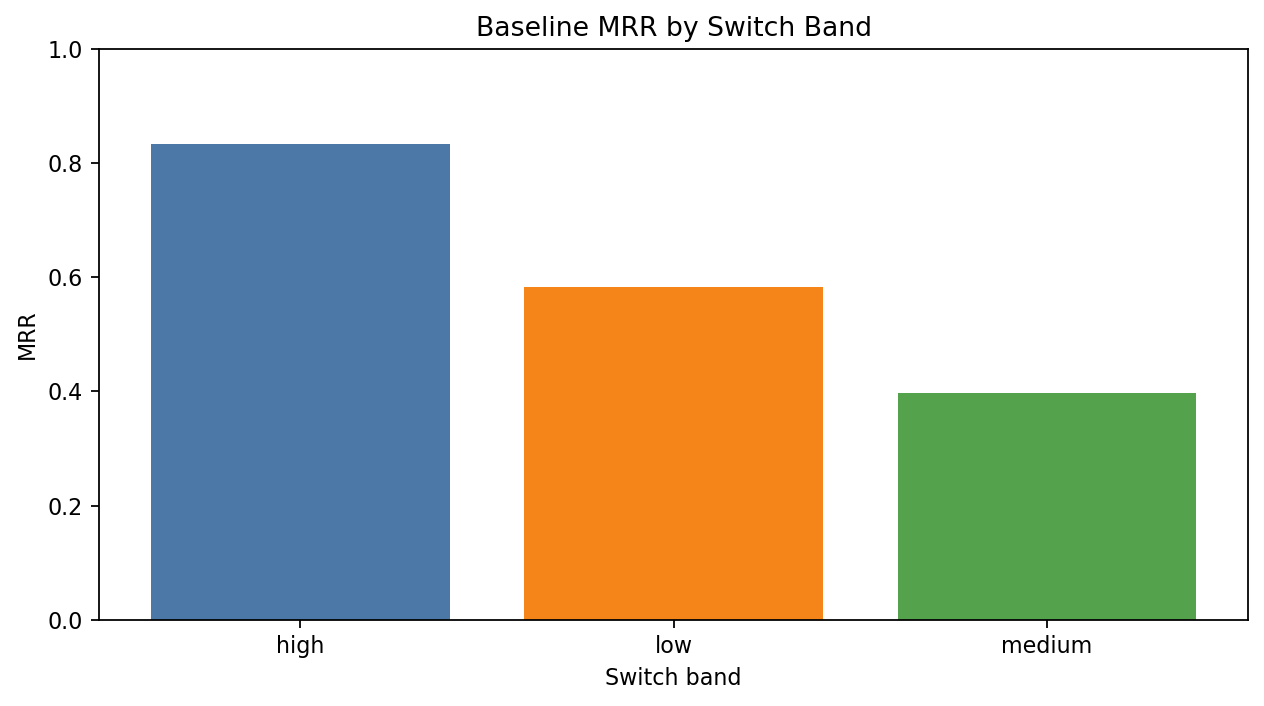
\includegraphics[width=\columnwidth]{experiment_outputs/plots/baseline_mrr_by_switch_band.png}
\caption{MRR by switch band on the original benchmark. The high-switch subset contains only three queries.}
\label{fig:switchband}
\end{figure}

Figure~\ref{fig:switchband} breaks performance down by switch band. The raw MRR values are 0.5837 for low-switch, 0.3976 for medium-switch, and 0.8333 for high-switch. The high-switch result looks best, but it is the least reliable result because it comes from only three queries. The more stable pattern is the drop on the medium-switch subset, where Recall@1 falls to 0.1429. On this benchmark, medium-switch items are the hardest condition.

\begin{figure}[t]
\centering
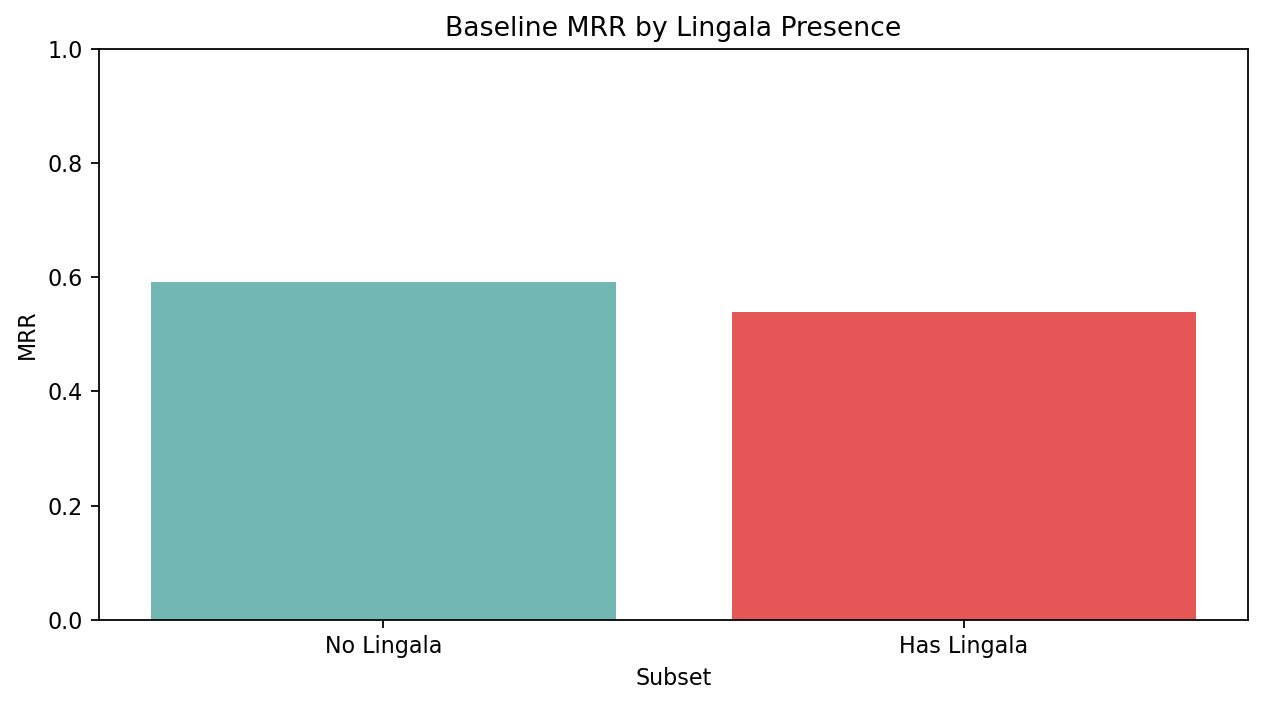
\includegraphics[width=\columnwidth]{experiment_outputs/plots/baseline_mrr_by_lingala_presence.png}
\caption{Lingala-bearing queries are slightly harder for the original lexical baseline.}
\label{fig:lingala}
\end{figure}

Figure~\ref{fig:lingala} shows a smaller but consistent gap by Lingala presence. Queries without Lingala reach 0.5912 MRR and 0.4154 Recall@1. Queries with Lingala drop to 0.5385 MRR and 0.3824 Recall@1. The bootstrap confidence interval for the MRR gap crosses zero, so this is a descriptive pattern, not a secure difference on the current sample.

\subsection{Dual-Track Matrix Results}
Table~\ref{tab:dualmatrix} reports the full 3$\times$3 matrix. The mixed Track~A+B pool gives the best French-dominant performance at 0.7800 MRR. Lingala-dominant non-French queries score best on Track~A at 0.8539 MRR, while Swahili-dominant non-French queries score best on Track~B at 0.8650 MRR.

\begin{table*}[t]
\centering
\small
\caption{Dual-track 3$\times$3 retrieval matrix with TF-IDF word-bigram retrieval.}
\label{tab:dualmatrix}
\begin{tabular}{@{}llrrrr@{}}
\toprule
Query language & Search corpus & Queries & MRR & Recall@1 & nDCG@5 \\
\midrule
French-dominant & Track A & 740 & 0.5609 & 0.4676 & 0.5513 \\
French-dominant & Track B & 740 & 0.5505 & 0.4662 & 0.5367 \\
French-dominant & Track A+B & 740 & 0.7800 & 0.6986 & 0.7925 \\
Lingala-dominant non-French & Track A & 395 & 0.8539 & 0.8076 & 0.8599 \\
Lingala-dominant non-French & Track B & 395 & 0.2489 & 0.1190 & 0.2192 \\
Lingala-dominant non-French & Track A+B & 395 & 0.7499 & 0.6658 & 0.7628 \\
Swahili-dominant non-French & Track A & 385 & 0.2588 & 0.1169 & 0.2325 \\
Swahili-dominant non-French & Track B & 385 & 0.8650 & 0.8234 & 0.8687 \\
Swahili-dominant non-French & Track A+B & 385 & 0.7919 & 0.7117 & 0.8047 \\
\bottomrule
\end{tabular}
\end{table*}

\begin{figure*}[t]
\centering
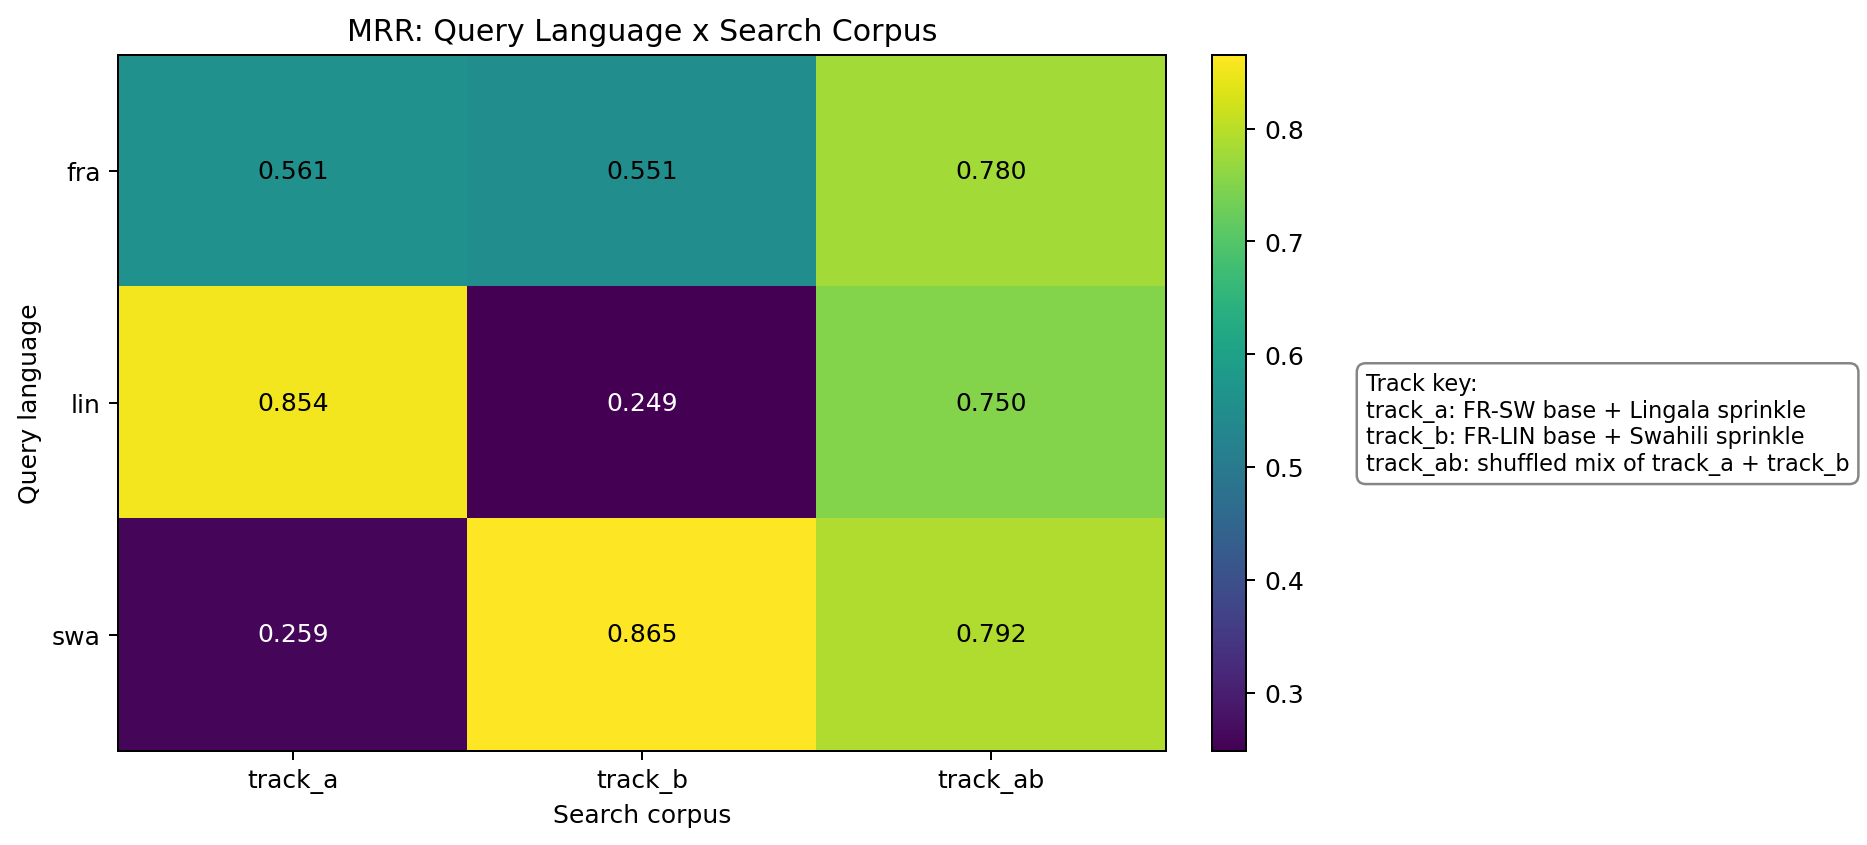
\includegraphics[width=0.85\textwidth]{experiment_outputs/dual_track/plots/dual_mrr_heatmap.png}
\caption{Dual-track MRR heatmap across query-language subsets and search corpora.}
\label{fig:dualheat}
\end{figure*}

The matrix is asymmetric. French-dominant queries score highest on the mixed pool. Lingala-dominant non-French queries score highest on Track~A. Swahili-dominant non-French queries score highest on Track~B. This pattern comes from the cross-track gold mapping used in the evaluation. It does not mean that Track~A is inherently better for Lingala or that Track~B is inherently better for Swahili outside this setup.

The dual-track by-band analysis also differs from the original benchmark. The matrix contains only medium- and high-switch examples, so CSRS is undefined in this setup. That is an empirical property of the denser-switching generation strategy and the query-subset definition, not a reporting omission.

\subsection{Statistical Significance in the Dual-Track Setup}
Because the same dual-track query sets are evaluated against multiple search corpora, we can run paired tests there. Table~\ref{tab:sig} shows the key comparisons. For French-dominant queries, the mixed pool is significantly better than either single track. For Lingala-dominant non-French queries, Track~A is significantly better than both Track~B and Track~A+B. For Swahili-dominant non-French queries, Track~B is significantly better than both Track~A and Track~A+B.

\begin{table*}[t]
\centering
\small
\caption{Key dual-track paired significance comparisons. $\Delta$MRR is the mean paired difference.}
\label{tab:sig}
\begin{tabular}{@{}lrrl@{}}
\toprule
Comparison & Queries & $\Delta$MRR & McNemar $p$ on Recall@1 \\
\midrule
French: Track A+B $-$ Track A & 740 & 0.2190 & $< 10^{-20}$ \\
French: Track A+B $-$ Track B & 740 & 0.2294 & $< 10^{-20}$ \\
Lingala: Track A $-$ Track B & 395 & 0.6051 & $< 10^{-20}$ \\
Lingala: Track A $-$ Track A+B & 395 & 0.1040 & $< 10^{-12}$ \\
Swahili: Track B $-$ Track A & 385 & 0.6062 & $< 10^{-20}$ \\
Swahili: Track B $-$ Track A+B & 385 & 0.0731 & $< 10^{-11}$ \\
\bottomrule
\end{tabular}
\end{table*}

These tests support two claims and only two claims. First, the matrix differences are not sampling noise inside the current dual-track setup. Second, the evaluation design matters. They do \emph{not} justify a broader claim that Track~A is universally better for Lingala or that Track~B is universally better for Swahili outside this setup.

\section{Error Analysis}
We manually inspected the 20 worst failed queries from the original benchmark, using the exported per-query ranks and the paired gold texts. Because the current CSV export stores rank metrics but not the top-ranked distractor text, this analysis focuses on what makes the gold pair hard rather than on the full ranked list. Even with that limitation, the failure patterns are clear.

We observed three recurring categories. First, 7 of the 20 failures are orthographic near-duplicates, where the query and gold differ by light suffix noise such as \emph{routes} versus \emph{routese} or \emph{annee} versus \emph{anneee}. Second, 4 failures are same-template lexical substitutions, where the overall topic remains the same but one or two content words shift. Third, 9 failures are switch-token mismatches involving inserted forms such as \emph{soki}, \emph{bazali}, \emph{batu}, or \emph{ndenge}. These tokens preserve enough surface overlap to confuse a lexical retriever while still changing which paired item is correct.

\begin{table}[t]
\centering
\caption{Representative failure cases from the original benchmark.}
\label{tab:errors}
\begin{tabular}{@{}p{0.46\columnwidth}p{0.46\columnwidth}@{}}
\toprule
Query & Gold \\
\midrule
\emph{Mkutano wa hadhara ulifanyika jana soir.} & \emph{Mkutanoe wa hadhara ulifanyika jana soir.} \\
\multicolumn{2}{@{}p{\columnwidth}@{}}{\textbf{Category:} orthographic near-duplicate.} \\
\addlinespace[0.4ex]
\emph{Serikali bazali mpango programme wa ajira kwa vijana.} & \emph{Serikali ilitangaza mpango programmee wa ajira ndenge vijana.} \\
\multicolumn{2}{@{}p{\columnwidth}@{}}{\textbf{Category:} same-template lexical substitution.} \\
\addlinespace[0.4ex]
\emph{budget ya afya imeongezeka mwaka huu.} & \emph{budget ya afya bazali soki huu.} \\
\multicolumn{2}{@{}p{\columnwidth}@{}}{\textbf{Category:} switch-token mismatch.} \\
\bottomrule
\end{tabular}
\end{table}

These errors show that the benchmark is not trivial. The model is not simply failing on unrelated negatives. It is often unable to separate highly similar candidates that share almost all of their lexical mass. That is exactly the type of behavior the benchmark was designed to expose.

The dual-track matrix adds a second error pattern. When the gold item comes from the complementary track, a lexical retriever can rank a same-track neighbor above it because the same-track neighbor shares more surface words. This is a limitation of the baseline, and it is also a direct consequence of the dual-track evaluation design.

\section{Discussion}
The results support three conclusions. First, the original benchmark is usable. The candidate pools are fixed, the metrics are exported, and the lexical baseline produces both correct matches and interpretable failures. Second, the original benchmark is not trivial. The baseline reaches 0.5803 MRR, but it still fails often on near-duplicate and switch-token cases. Third, the current numbers apply only to this synthetic dataset.

The dual-track evaluation answers a different question. It asks how the same lexical retriever behaves when the query is compared against three search pools built from two complementary generation tracks. In that setup, the mixed pool helps French-dominant queries, Track~A helps Lingala-dominant non-French queries, and Track~B helps Swahili-dominant non-French queries. The paired tests show that these differences are real inside this matrix.

The matrix does not support a broader claim about language difficulty by itself. Its preferred gold mapping is cross-track. Because of that choice, some high scores reflect successful retrieval of complementary formulations, and some low scores reflect competition from closer same-track neighbors. This is useful evidence about the dataset and the evaluation design. It is not a final statement about real-world multilingual retrieval in eastern DRC.

\subsection{Real-Data Source Assessment}
Recent Congolese speech resources improve the next stage of this project \cite{kimanuka2024speech,kimanuka2023mendeley,ussen2024cdwav2vec}. Those releases include multiple Congolese languages, including Lingala, Tshiluba, Kikongo, and Congolese Swahili. In this project, we focused only on the Congolese Swahili portion because it is the closest match to our target setting.

Athanase Bahizire manually reviewed 20 random Congolese Swahili recordings from the Mendeley-linked corpus. He is a native speaker. In those samples, the speech was mostly Swahili, with French insertions and lighter Lingala use. That pattern is broadly consistent with the multilingual direction assumed by the synthetic pipeline.

This source also has a clear limitation. The audio comes from broadcast media. Some segments contain only music. Other segments are so music-dominant that they are not useful for retrieval or ASR benchmarking without cleaning. For that reason, the usable Congolese Swahili subset may be much smaller than the raw duration suggests. More data is still needed, and some of that data should come from sources other than broadcast media.

\section{Future Work}
The most important next step is to obtain a stronger real local voice dataset from eastern DRC. We already prepared the community-collection path because a realistic benchmark will eventually require real speakers from places such as Goma and Bukavu, not only synthetic renderings. That future dataset should better capture the fluid way local speakers move across Swahili, French, and Lingala within a single utterance.

The next experimental phase should do four things. First, it should rebuild the text splits to remove source-family leakage. Second, it should evaluate the mixed Track~A+B corpus with stronger text encoders such as SERENGETI and AfriBERTa \cite{serengeti,afriberta}. Third, it should move to cross-modal retrieval with CLAP-style or related audio-text alignment methods \cite{elizalde2019crossmodal,nuga2025multilingual}. Fourth, it should connect cleaned real-data sources, including the most relevant Congolese Swahili material from the new corpora, to the same evaluation protocol.

We also discussed a broader resource-survey direction with a CMU-Africa alumni who are already conducting comprehensive language-resource surveys for their own languages. We are considering doing a similar survey for Congolese Swahili and closely related DRC multilingual resources over the summer. That survey could become the basis of a publishable paper because the available resources are still scattered across papers, repositories, and community datasets.

\section{Conclusion}
This report turns the project into a working benchmark and a measurable stress test. The original benchmark is usable, and the TF-IDF baseline reaches an MRR of 0.5803 and a Recall@1 of 0.4085. The failures are systematic, not random. Near-duplicate strings, template-level substitutions, and switch-token mismatches account for the hardest cases. That error pattern shows that the benchmark captures the ambiguity that a retrieval system must handle.

The dual-track extension adds a clearer stress test. The mixed Track~A+B pool raises retrieval across the three query groups, with MRR of 0.7800 and Recall@1 of 0.6986 for French-dominant queries, MRR of 0.7499 and Recall@1 of 0.6658 for Lingala-dominant non-French queries, and MRR of 0.7919 and Recall@1 of 0.7117 for Swahili-dominant non-French queries. That result makes the dual-track design useful, not just larger. The project is still synthetic, but it now gives us a concrete benchmark, interpretable scores, and a clearer next step toward real Congolese Swahili speech data.

\bibliographystyle{plain}
\bibliography{reference}

\appendix
\section{Contribution Statement}
For this report, many tasks were done collaboratively. We jointly designed the project scope, defined the corpus construction strategy, decided the benchmark protocol, interpreted the results, and wrote the main narrative of the paper together.

Athanase led the report revision, benchmark framing, and the review of the Mendeley-linked Congolese Swahili audio resource as a native speaker. Stephen led the corpus generation pipeline, data organization, and the supporting engineering around the collection workflow and released artifacts. The dual-track experiment was implemented sequentially together, with both authors reviewing the outputs and their interpretation. The final report integrates both contributions.

\end{document}
